\chapter{Case Study} \label{cpt-case-study}

Our case study is based on an implementation within the framework \emph{Diligent Engine}.[@TODO: cite DiligentEngine]
This framework includes a multi-\ac{API} rendering backend, with modern integrations for \ac{GPU}-driven rendering.
One of these modern features is the support for mesh shading in Microsoft's D3D12 rendering \ac{API}. 
The support for modern rendering features while still maintaining access to all core features, makes 
\emph{Diligent Engine} a good place to start from. For the case study, we enhanced the mesh shading pipelin 
to better fit our purposes of drawing a huge amount of voxels. We also made small changes to the integrated 
view-frustum culling, which was updated to work on meshlet-groups rather than meshlets themselves. This change 
was made during the restructuring of the draw tasks. The updated pipeline changes how meshes are dispatched 
because of the use of additional acceleration structures. This chapter provides an overview of all the changes and 
additions to the framework and how the pipeline works in specific. The implementation details can be found in the 
appendix \ref{cpt-appendix}.

\section{Pipeline Overview}

\begin{figure}[h]
    \centering
    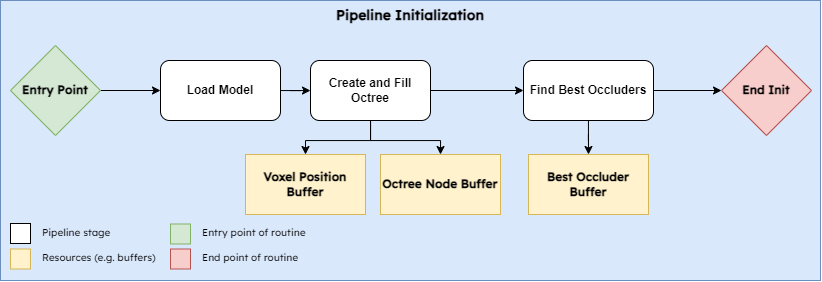
\includegraphics[width=\linewidth]{images/graphics/pipeline-initialization.png}
    \caption{The initialization process of the rendering pipeline. }
    \label{fig:pipeline-initialization}
\end{figure}


\begin{figure}[h]
    \centering
    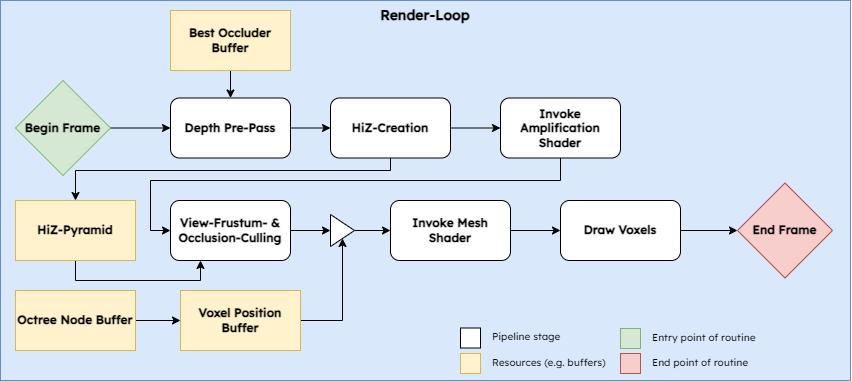
\includegraphics[width=\linewidth]{images/graphics/render-loop.png}
    \caption{The rendering loop of the rendering pipeline. }
    \label{fig:pipeline-loop}
\end{figure}


% @TODO: Meshlet Creation -> Voxel

- Meshlet creation for voxel meshes is trivial since meshlets don't have to be per-computed
- Meshlet culling is also straight forward since Voxels are inherently AABBs
- 

\section{Setup}

% @TODO: Add reference to Diligent Engine's github etc.
For the case study, a starting point is used which provides a reliable and comparable environment.
The framework used is the \emph{Diligent Engine} which already implements state of the art, multi-
platform and multi-API rendering. \\

\noindent



// --------------------------------------------------------------------------------- //
Motivation:
Use Meshlet Culling in voxel rendering to optimize GPU Driven Voxel Rendering


Implementation Considerations:

- Meshlet Culling at first, then problem, because meshlet culling algorithm depends on different algos
    - Meshlet Backface Culling -> Not possible because Meshlets are voxels in this case
    - Meshlet Occlusion Culling -> Using 2 Pass Depth Occlusion Culling sounds good!
    - 2PDOC relies on drawing best occluders which are usually hand picked by artists (buildings)
        -> We can dynamically pick best occluders by selecting full octree nodes as best occluders!

- Optimize octree by using High Res SVOs (https://www.cse.chalmers.se/~uffe/HighResolutionSparseVoxelDAGs.pdf).
    - As shown in the paper, here we also only need to encode if a node is filled or not. This way we can 
    optimize memory and proccessing speed! (Not done here because of limitation in loading and voxelizing models.)

- Explain why Mesh Shading is useful here and what the differences to HiZ and Two-Pass OC are!

- Align octree bounds with outer most voxel bounds, so no misalignment happens!
    
- Limitations: 
    - Using Mesh Shading, we occlude meshlets against other meshlets, instead of instances against other
    instances. This might be a limiting factor!

- Worse performance on slopes? -> Check and measure!

- Larger nodes which are not being split can be "full" without being full!

// --------------------------------------------------------------------------------- //
